\chapter{Auswertung}
\label{ch:Auswertung}
% Liste der genutzer Formeln für die Fehlerrechnung
\section*{Fehlerrechnung}
Für die statistische Auswertung von $n$ Messwerten $x_i$ werden folgende Größen definiert \cite{errorSkript25}:
\begin{align}
    \bar{x} &= \frac{1}{n} \sum_{i=1}^{n} x_i \vphantom{\sqrt{\sum_i^n}^2} && \text{\textcolor{gray}{Arithmetisches Mittel}} \label{eq:arithmetisches_mittel} \\
    \sigma^2 &= \frac{1}{n-1} \sum_{i=1}^{n} (x_i - \bar{x})^2 \vphantom{\sqrt{\sum_i^n}^2} && \text{\textcolor{gray}{Varianz}} \label{eq:Varianz} \\
    \sigma &= \sqrt{\frac{1}{n-1} \sum_{i=1}^{n} (x_i - \bar{x})^2} \vphantom{\sqrt{\sum_i^n}^2} && \text{\textcolor{gray}{Standardabweichung}} \label{eq:standardabweichung} \\
    \Delta \bar{x} &= \frac{\sigma}{\sqrt{n}} = \sqrt{\frac{1}{n(n-1)} \sum_{i=1}^n(\bar x - x_i)^2} \vphantom{\sqrt{\sum_i^n}^2} && \text{\textcolor{gray}{Fehler des Mittelwerts}} \label{eq:fehler_mittelwert} \\
    \Delta f &= \sqrt{\left(\frac{\partial f}{\partial x} \Delta x\right)^2 + \left(\frac{\partial f}{\partial y} \Delta y\right)^2} \vphantom{\sqrt{\sum_i^n}^2} && \text{\textcolor{gray}{Gauß’sches Fehlerfortpflanzungsgesetz für $f(x,y)$}} \label{eq:gauss_fehlfortpflanzung} \\
    \Delta f &= \sqrt{(\Delta x)^2 + (\Delta y)^2} \vphantom{\sqrt{\sum_i^n}^2} && \text{\textcolor{gray}{Fehler für $f = x + y$}} \label{eq:fehler_summe} \\
    \Delta f &= |a| \Delta x \vphantom{\sqrt{\sum_i^n}^2} && \text{\textcolor{gray}{Fehler für $f = ax$}} \label{eq:fehler_proportional} \\
    \frac{\Delta f}{|f|} &= \sqrt{\left(\frac{\Delta x}{x}\right)^2 + \left(\frac{\Delta y}{y}\right)^2} \vphantom{\sqrt{\sum_i^n}^2} && \text{\textcolor{gray}{relativer Fehler für $f = xy$ oder $f = x/y$}} \label{eq:relativer_fehler} \\
    \sigma &= \frac{|a_{lit} - a_{gem}|}{\sqrt{\Delta a_{lit}^2 + \Delta a_{gem}^2}} \vphantom{\sqrt{\sum_i^n}^2} && \text{\textcolor{gray}{Berechnung der signifikanten Abweichung}} \label{eq:signifikante_abweichung}
\end{align}

\newpage
In diesem Kapitel sollen die aufgenommenen Spektren untersucht und ausgewertet werden. Im \cch{Diskussion} werden die Ergebnisse dann Diskutiert. 
Es ist anzumerken, dass dem Anhang (\cch{Anhang}) die direkt aufgenommenen Bilder zu entnehmen sind. In der Auswertung werden die Spektren in Python geplottet.

\section{Untersuchung des Sonnenspektrums}
\label{sec:A1}
\subsection{Einfluss der Fensterscheibe auf das Sonnenlichtspektrum}
In dieser Sektion soll das Spektrum der Sonne untersucht werden. Insbesondere soll der Einfluss einer Fensterscheibe auf das Spektrum untersucht werden. Daher wurden zwei Messreihen aufgenommen, eine durch die Fensterscheibe hindurch und eine durch das geöffnete Fenster. Die Resultate sind der \cabb{A1/Vergleich_Sonnenspektren_1a} zu entnehmen.
\img[1]{A1/Vergleich_Sonnenspektren_1a}{Plot der beiden Intensitäten gegen die jeweilige Wellenlänge des Sonnenlichtes.}
Dem Plot ist zu entnehmen, dass die Fensterscheibe einen Einfluss auf die Intensität des Sonnenlichtes hat, diese wird abgeschwächt. Die allgemeine Struktur beider Fälle bleibt jedoch erhalten. So liegen beide Maxima bei $\approx (520\pm5) \mathrm{nm}$. Die durchschnittle Abschwächung der Intensität beträgt dabei $\approx 21.67\%$. Diese wurde über dasm \hyperref[eq:arithmetisches_mittel]{arithmetische Mittel (\ref*{eq:arithmetisches_mittel})} geildet. Die Abweichung ist jedoch stark von der Wellenlänge abhänig. Dies ist an dem \hyperref[eq:fehler_mittelwert]{Fehler des Mittelwertes (\ref*{eq:fehler_mittelwert})} gut zu erkennen, welcher $38.33\%$ beträgt. 
Zur untersuchung der Absorptions in Abhänigkeit der Wellenlänge wird nicht das \hyperref[eq:arithmetisches_mittel]{arithmetische Mittel (\ref*{eq:arithmetisches_mittel})} der prozentualen Abweichung gebildet, sondern an jeder Stelle der Wert verglichen. Dies ist mathematisch über
\eq{absorptions_rel}{
    A_\text{Glas}(\lambda) = 1 - \frac{I_\text{ges}(\lambda)}{I_\text{offen}(\lambda)} 
}
beschrieben. Die \ceq{absorptions_rel} ist dabei in \cabb{A1/Abs_S_1b} geplottet dargestellt. 
\img[1]{A1/Abs_S_1b}{Plot der relativen Absorption durch die Fensterscheibe. Eingezeichnet ist zudem der für Menschen sichtbare Bereich.}

Es ist zu beobachten, dass die Absorption in dem Infrarot-, sowie dem ultraviolettem Bereich am größten ist. In den sichtbaren bereich ist die absorption am geringsten. Dies entspricht der Erwartung an ein (für Menschen) durchsichtiges Material. 
Da die Fensterscheibe dementsprechend Teile des Lichtes\afz{Stört}, soll im weiteren Verlauf nur Messreihe ohne Fensterscheibe betrachtet werden; Hier können dann die Einflüsse der Athmosphäre auf das Spektrum betrachtet werden.


\subsection{Bestimmung der Frauenhofer Linien}
In dieser Sektion wird das gemessene Sonnenlichtspektrum ohne Fensterscheibe analisiert. Betrachtet man das gemessene Spektrum und vergleicht es mit dem theoretischen Spektrum nach \cabb{intVert_schwarzerKoerper}, so fallen einige\afz{Einkärbungen} in dem Spektrum auf. 
Dies sind die Frauenhofer Linien, welche durch die Wechselwirkung von Luftmolekühlen und dem Licht entstehen. Eine Nummerische Bestimmung der Frauenhofer Linien etwa via Python stellt sich Aufgrund des Rauschen des Signals als herausfordern heraus. 
% \wrap[0.5]{R}{Frauenhoferlinien_Eingezeichnet_MitMessurments}{Gespeicherter Plot mit händisch eingezeichneten Frauenhofer Linien, sowie die relativen Distanzen,  bestimmt von Inkscape.}
\img[0.75]{Frauenhoferlinien_Eingezeichnet_MitMessurments}{Gespeicherter Plot mit händisch eingezeichneten Frauenhofer Linien, sowie die relativen Distanzen,  bestimmt von Inkscape.}
Daher wurden die peaks händisch, bzw. visuell bestimmt. Dafür wurde der in Python erstellte Plot als PDF in die Grafiksoftware\afz{Inkscape} importiert. Da in Inkscape die Elemente Vektorbasiert sind, geht beim transferieren des Plots keine Information Aufgrund der Auflösung verloren. 
Zudem ist das heranzoomen an Plot positionen problemlos möglich, da auch hier keine Informationen durch die Auflösung verloren gingen. Die Dicke der Plotlinie wurde ebenfalls angepasst, um nah beieinander liegende Punkte unterscheiden zu können.
Die Positionen der Linien wurden dann über das integrierte Vermessungs Tool von Inkscape vermessen. Der in Inkscape manipulierte Plot ist der \cabb{Frauenhoferlinien_Eingezeichnet_MitMessurments} zu entnehmen. 
Die Distanzen wurden in Inkscape in mm angegeben. Um diese Distanz in die tatsächlichen Wellenlängen in nm umzurechnen wird ein Skalierungsfaktor bestimmt, dieser beträgt $s_\text{ink} \approx 2.0 \mathrm{nm/mm}$. Wichtig dabei ist, dass mm hier die von Inkscape bestimmte theoretische Distanz ist, wenn das Dokument gedruckt wäre und man physisch die Abstände messen würde. Die Einheit nm entspricht dabei der physikalischen Wellenlänge des Lichts.
Für die Bestimmung der Frauenhofer Linien wurde die Ungenauigkeit von $\Delta \text{Ink} = 0.15 \mathrm{mm}$ abgeschätzt, bzw. von $\Delta \lambda \approx 0.3 \mathrm{nm}$. Die Ergebnisse sind der \cabb{A1/FL_S_1c} zu entnehmen. 
Die Messergebnisse wurden mit den theoretischen Werten verglichen. \cite{wikiFL}
\img{A1/FL_S_1c}{Ausschnitt des Sonnenlichtspektrums mit den Positionen der vermessenen Frauenhofer Linien.}
Die Namen der bestimmten Frauenhofer Linien sind bereits in dem Plot gegeben. Die nummerisch bestimmten Frauenhofer Linien, sowie die theoretischen Werte sind inklusive der \hyperref[eq:standardabweichung]{Standardabweichung (\ref*{eq:standardabweichung})} zwischen experimentellen und theoretischen Werten der \ctab{fraunhofer} zu entnehmen.

\begin{table}[h!]
    \caption{Vergleich der theoretischen und experimentellen Frauenhofer-Linien. Grün gekennzeichnet sind die Elemente der Balmer-Serie}
    \label{tab:fraunhofer}
    \centering
    \begin{tabular}{l | C C || C}
        \toprule
        \text{Line} & \lambda_\text{theo} [\mathrm{nm}] & \lambda_\text{exp} [\mathrm{nm}] & \text{Std. Abw. } \sigma \\
        \midrule
        $K$ & 393.4 & 392.9 \pm 0.3 & 1.8 \\
        $H$ & 396.8 & 396.2 \pm 0.3 & 2.2 \\
        \cellcolor{GreenTri}$h / H_\delta$ & \cellcolor{GreenTri}410.2 & \cellcolor{GreenTri}409.2 \pm 0.3 & \cellcolor{GreenTri}3.2 \\
        $G$ & 430.8 & 430.0 \pm 0.3 & 2.6 \\
        \cellcolor{GreenTri}$G' / H_\gamma$ & \cellcolor{GreenTri}434.0 & \cellcolor{GreenTri}433.8 \pm 0.3 & \cellcolor{GreenTri}0.6 \\
        \cellcolor{GreenTri}$F / H_\beta$ & \cellcolor{GreenTri}486.1 & \cellcolor{GreenTri}485.8 \pm 0.3 & \cellcolor{GreenTri}1.0 \\
        $b_2$ & 517.3 & 516.5 \pm 0.3 & 2.5 \\
        $b_1$ & 518.4 & 517.8 \pm 0.3 & 2.0 \\
        $E$ & 527.0 & 526.5 \pm 0.3 & 1.6 \\
        $D_2$ & 589.0 & 588.6 \pm 0.3 & 1.2 \\
        $D_1$ & 589.6 & 589.0 \pm 0.3 & 1.9 \\
        \cellcolor{GreenTri}$C / H_\alpha$ & \cellcolor{GreenTri}656.3 & \cellcolor{GreenTri}655.9 \pm 0.3 & \cellcolor{GreenTri}1.4 \\
        $B$ & 686.7 & 687.0 \pm 0.3 & 1.0 \\
        $A$ & 759.4 & 760.4 \pm 0.3 & 3.5 \\
        \bottomrule
    \end{tabular}
\end{table}

\textcolor{red}{Vielleicht den folgenden Teil in die Diskussion verschieben:}
\subsubsection*{Einschub: Doppelte Linien}
% \wrap[0.45]{L}{A1/bL_1Z}{Ausschnitt an die $b_1$ und $b_2$ Linien.}
% \wrap[0.45]{R}{A1/DL_1Z}{Ausschnitt an die $D_1$ und $D_2$ Linien.}
An dieser Stelle ist es wichtig zu betonen, dass die theoretischen Werte der Frauenhofer Linien vor und während der Bestimmung der Frauenhofer Linien in Inkscape dem Experimentator bekannt waren und dieser somit einem Bais unterlag. 
\begin{figure}[h!]
    \centering
    \begin{minipage}{0.49\textwidth}
        \centering
        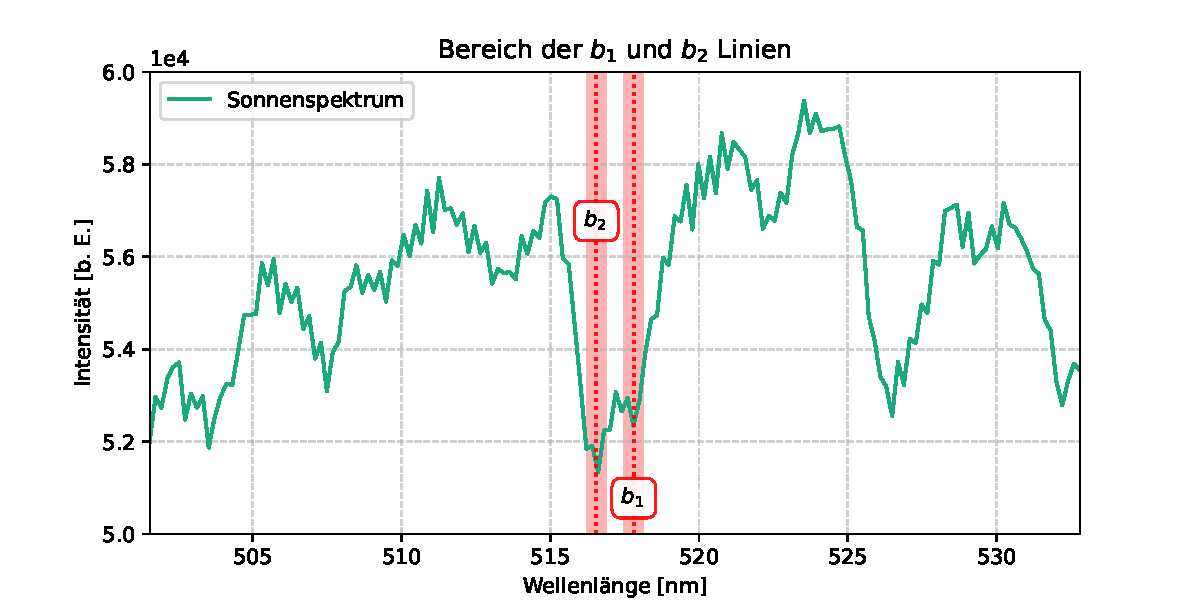
\includegraphics[width=\textwidth]{Versuche/234/img/A1/bL_1Z.pdf}
    \end{minipage}
    \hfill
    \begin{minipage}{0.49\textwidth}
        \centering
        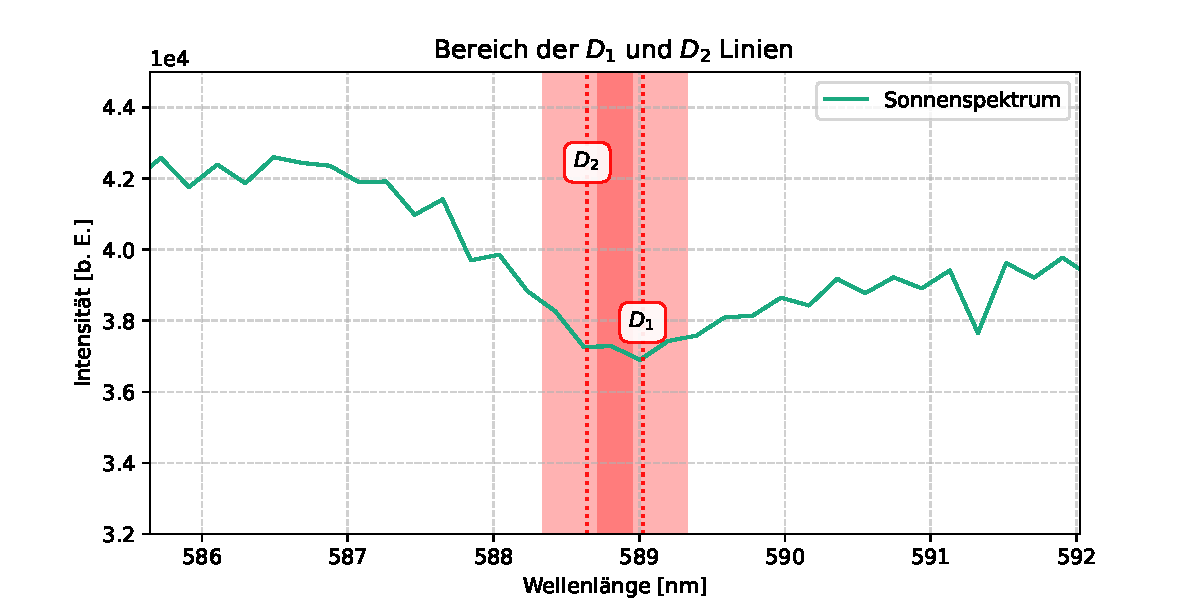
\includegraphics[width=\textwidth]{Versuche/234/img/A1/DL_1Z.pdf}
    \end{minipage}
    \caption{Ausschnitte an die jeweiligen Bereiche der $b$- bzw. $D$-Linien.}
    \label{fig:DbL}
\end{figure}
Dies ist insbesondere bei den Linien $b_1$ und $b_2$, sowie bei den Linien $D_1$ und $D_2$ ein Problem, da diese besonders nah beieinander liegen. Daher werden diese beiden bereiche noch einmal explizit untersucht. 
Dafür werden die \hyperref[eq:standardabweichung]{Standardabweichung (\ref*{eq:standardabweichung})} zwischen den jeweiligen Werten bestimmt. Für die $b$-Linien stellt sich eine standardabweichung von $3.0\sigma$ ein, dies entspricht einer signifikanten Abweichung. Somit lasst sich statistisch sagen, dass die Werte verschieden sind. 
Dies passt auch zu den visuellen Beobachtungen. Die \cabb{DbL} zeigt zum einen, dass tatsächlich zwei Peaks zu beobachten sind. Zudem lässt sich visuell gut erkennen, dass die Fehlerbereiche sich nicht überschneiden. 
Äquivalent werden die $D$-Linien untersucht. Für die \hyperref[eq:standardabweichung]{Standardabweichung (\ref*{eq:standardabweichung})} ergibt sich $0.9\sigma$, diese Abweichung ist nicht signifikant, daher lässt sich hier statistisch nicht sagen, dass es sich um verschiedene Werte handelt. 
Vergleichbares ist visuell festzustellen, die \cabb{DbL} zeigt, dass sich die Fehlerbereiche der beiden Linien überschneiden, zudem sind keine eindeutigen Peaks\footnote{Die hier gezeigten könnten einfache Fluktuationen des Messsignals sein.} festzustellen. 

Dies zeigt, dass der Experimentator hier mutmaßlich tatsächlich einem Bais unterlag. Es lassen sich keine zwei verschiedenen $D$-Linen feststellen. Dies steht im Konflikt zur Theorie.


\section{Vergleich künstlicher Lichtquellen}
\label{sec:A2}
Nachdem in \csec{A1} eine natürliche Lichtquelle untersucht wurde, sollen hier künstliche Lichtquellen untersucht werden, welche auf unterschiedliche Weisen funktionieren und unterschiedliche Lichtspektren aufweisen. Die Signale, die untersucht werden sind der \cabb{A2/Spektren_Grid} zu entnehmen.
\img[1]{A2/Spektren_Grid}{Übersicht aller 12 Signale, welche untersucht werden.}

Von allen zwölf Signalen soll die mittlere Wellenlänge $\overline{\lambda_n}$ bestimmt werden. Diese berechnet sich über
\eq{abg_wavL}{
    \overline{\lambda_n} = \frac{\sum_i \lambda_{n,i} \, I_{n,i}}{\sum_i I_{n,i}} \, .
}

Die nach \ceq{abg_wavL} berechneten Wellenlängen $\overline{\lambda_n}$ sind der \ctab{wellenlaengen} zu entnehmen.
\begin{table}[h!]
    \caption{Mittlere Wellenlängen verschiedener Lichtquellen}
    \label{tab:wellenlaengen}
    \centering
    \begin{tabular}{l | c}
        \toprule
        Lichtquelle & Mittlere Wellenlänge [nm] \\
        \midrule
        LED warmweiß & 586.02 \\
        LED kaltweiß & 582.23 \\
        LED blau & 466.89 \\
        LED weiß & 543.59 \\
        LED orange & 608.02 \\
        LED gelb & 592.27 \\
        LED rot & 627.85 \\
        Energiesparlampe & 588.27 \\
        Glühlampe & 650.26 \\
        Laser & 532.13 \\
        LED Hue RGB & 611.67 \\
        LED Lampe & 580.95 \\
        \bottomrule
    \end{tabular}
\end{table}
Im Folgenden sollen jene Lichtquellen qualitativ untersucht und verglichen werden. Es werden vier verschiedene Eigenschaften untersucht, wleche anhand der \cabb{A2/Vgl_LQ_2c} erleutert werden.
Dabei ist wichtig, dass die Intensitäten nicht vergleichbar sind, es kann lediglich die Struktur verglichen werden.

\paragraph{c) Weiße LEDs}
In diesem Plot sind die Spektren dreier LEDs dargestellt. Diese unterscheiden sich in ihrer\afz{Wärme}. Dabei beschreibt\afz{warmes Licht} ein rötlicheres Licht als, und\afz{kaltes Licht} ein bläuliches Licht. Dabei ist die\afz{Basis} weißes Licht.
Genau dies ist auch dieser Abbildung zu entnehmen. In dem Wellenlängen bereich von $420-490 \mathrm{nm}$ befindet sich das sichtbare blaue Licht. Es zeigt sich, je wärmer das Licht ist, desto größer ist die Intensität in diesem Wellenlängen bereich. 
Im Bereich von $500-700 \mathrm{nm}$ befindet sich dann das Spektrum, welches besagte weiße Basis darstellt.

\paragraph{d) Einfarbige LEDs}
In diesem Plot sind vier Spektren von einfarbigen LEDs dargestellt. Es zeigt sich, dass genau der Wellenlängenbereich eine hohe Intensität aufweist, in welcher die LED leuchet. Es handelt sich jedoch nicht wirklich um monochromatisches Licht, da immer noch ein Wellenlängenbereich abgedeckt wird.

\paragraph{a) Alle LEDs}
In diesem Plot sind die Unterschiede zwischen Weißen LEDs und einfarbigen LEDs zu erkennen. Die Farbigen LEDs bestehen nur aus dem breitem Peak, während die Spektren der weißen LEDs fast im gesmaten sichtbaren Bereich verteilt sind.

\paragraph{b) Verschiedene Lichtquellen}
In diesem Plot sind weitere Lichtquellen und deren Spektren dargestellt. Es lassen sich zwei\afz{Gruppe} erkennen. Erstens die schmalen Spektren, welche monochromatisch vom Menschen wahrgenommen werden und zweitens in die weißen Spektren. 
Zu den monochromatischen Lichtquellen gehöhren die einfarbigen LEDs und der LASER. Wichtig ist, dass der LASER tatsächlich annährend monochromatisch ist, während die LED ein breiteres Spektrum abdekt. Die Energiesparlampe ist in dem Spektrum zwar nicht direkt als monochromatisch zu benennen, aber weißt dennoch wenige schmale Peaks auf. Diese entstehen durch die Glühemission von Elektronen im Gas. Somit sind für verschiedene Leuchtmittel (Gase) auch unterschiedliche Spektren zu erwarten. 
Die zweite Gruppe sind die breiten Spektren, welche für den Menschen als weiß wahrgenommen werden. Hierbei unterscheiden sich die Farbtemperaturen wie bereits erwähnt über den jeweiligen blau- und rotanteil der Spektren. Damit ist auch klar, wieso die Glühlampe als\afz{warm} wahrgenommen wird, denn ein großer Teil des Spektrums weißt eine große Intensität im roten Licht bereich auf. Die LED dagegen wird als weißer bzw. kälter  wahrgenommen, da diese einen geringeren rotanteil hat. 
Zuletzt fällt auch auch, dass die LED primär Licht im sichtbaren Bereich ausstrahlt, während die Glühlampe auch im Infrarotbereich strahlt.

\img[1]{A2/Vgl_LQ_2c}{Überlagerung der untersuchten Lichtquellen nach verschiedenen Eigenschaften.}
\textcolor{red}{Reihenfolge der Plots anpassen und bei verschiedene Lichtquellen noch einfarbige LED hinzufügen}

\section{Das Natrium-Spektrum}
\label{sec:A3}
In dieser Sektion wird die Strahlung der Natriumdampflampe untersucht. Insbesondere sollen die Emissionslinien bestimmt werden. Dafür wurde das Spektrum in verschiedene Bereiche aufgeteilt, die unterschiedliche Bereiche betonen und die Untersuchung erleichtern sollen. Die Auswertung erfolgt dabei nummerisch via Pyhton. 
Später sollen die bestimmten Emissionslinien mit der Haupt und den beiden Nebenserien des Natriums verglichen werden. ( Vgl. \cabb{Na_Spektrum})
\subsection*{Bestimmen der Emissionslinien von Natrium}
Es wird eine Ungenauigkeit von $\Delta \lambda = 1.2 \mathrm{nm}$ angenommen. Die \cabb{A3/Na_Spektren_Grid_3c} zeigt Auschnitte aus dem Natriumspektrum und die bestimmten Emissionslinien. Bei dem Plot A ist den Experimentatoren ein Fehler aufgetreten, die linke Line (Line A1) ist in Sättigung. Dadurch ist der Wert größer bestimmt wurden.
Die bestimmten Wellenlängen stehen auf den Plots und sind der \ctab{Emissionslinien_Na} zu entnehmen.
\img[1]{A3/Na_Spektren_Grid_3c}{Emissionslinien der Natriumdampflampe in verschiedenen Wellenlängenbereichen.}

\begin{table}[h!]
    \caption{Gemessene Emissionslinien der Natriumlampe}
    \centering
    \label{tab:Emissionslinien_Na}
    \begin{tabular}{l | c | c || l | c | c || l | c | c}
        \toprule
        Bild & idx & Wellenlänge $\lambda$ [nm] & Bild & idx & Wellenlänge $\lambda$ [nm] & Bild & idx & Wellenlänge $\lambda$ [nm] \\
        \midrule
        A & 1 & $331.9 \pm 1.2$ & B & 1 & $415.5 \pm 1.2$ & C & 1 & $588.6 \pm 1.2$ \\
        & 2 & $498.1 \pm 1.2$ &  & 2 & $419.4 \pm 1.2$ &  &  &  \\
        & 3 & $515.0 \pm 1.2$ &  & 3 & $426.7 \pm 1.2$ &  &  &  \\
        &  &  &  & 4 & $433.0 \pm 1.2$ &  &  &  \\
        &  &  &  & 5 & $455.1 \pm 1.2$ &  &  &  \\
        &  &  &  & 6 & $466.3 \pm 1.2$ &  &  &  \\
        &  &  &  & 7 & $471.6 \pm 1.2$ &  &  &  \\
        &  &  &  & 8 & $493.0 \pm 1.2$ &  &  &  \\
        \midrule
        D & 1 & $568.4 \pm 1.2$ & E & 1 & $763.0 \pm 1.2$ & F & 1 & $695.9 \pm 1.2$ \\
        & 2 & $615.6 \pm 1.2$ &  & 2 & $772.0 \pm 1.2$ &  & 2 & $706.1 \pm 1.2$ \\
        &  &  &  & 3 & $811.1 \pm 1.2$ &  & 3 & $737.8 \pm 1.2$ \\
        &  &  &  & 4 & $819.2 \pm 1.2$ &  & 4 & $750.6 \pm 1.2$ \\
        &  &  &  &  &  &  & 5 & $765.9 \pm 1.2$ \\
        &  &  &  &  &  &  & 6 & $769.3 \pm 1.2$ \\
        &  &  &  &  &  &  & 7 & $794.3 \pm 1.2$ \\
        &  &  &  &  &  &  & 8 & $800.9 \pm 1.2$ \\
        &  &  &  &  &  &  & 9 & $825.9 \pm 1.2$ \\
        &  &  &  &  &  &  & 10 & $841.9 \pm 1.2$ \\
        &  &  &  &  &  &  & 11 & $852.2 \pm 1.2$ \\
        \bottomrule
        \end{tabular}
\end{table}


\subsection*{Erste Nebenserie}
In diesem Abschnitt wird bestimmt, welche gemessenen Wellenlängen zur ersten Nebenserie des Natriums gehöhren. Dafür werden die theoretisch erwarten Wellenlängen nach \ceq{neben1} bis zur Hauptquantenzahl $m = 12$ bestimmt. 
Dafür muss jedoch $E_{3p}$ ermitttelt werden. Dazu wird die Wellenlänge gesucht, welche dem Übergang von $3d$ nach $3P$ entspricht. Diese Eigenschaft erfüllt die Linie E4 mit $\lambda_\text{E4} = (819.2 \pm 0.6) \mathrm{nm}$. \ceq{neben1} wird nach $E_{3p}$ aufgelöst, und mit $m=3$ gelöst. Die Gleichung und die dazugehörige Ungenauigkeit nach \hyperref[eq:gauss_fehlfortpflanzung]{Gauß'scher Fehlerfortpflanzung (\ref*{eq:gauss_fehlfortpflanzung})} lauten
\eq{E_drei_pe}{
    E_{3p} = \frac{-E_\text{Ry}}{3^2} - \frac{h\,c}{\lambda_\text{E4}} \, ,  \qquad  \Delta E_{3p} = \frac{h\,c}{{\lambda_\text{E4}}^2} \, \Delta \lambda_\text{E4} \, .
}
Durch einsetzen aller bekannten Werte ergibt sich 
\res{E_{3p}}{-3.0251}{0.0022}{eV}

Die ungenauigkeit von \ceq{neben1} berechnet sich nach \hyperref[eq:gauss_fehlfortpflanzung]{Gauß'scher Fehlerfortpflanzung (\ref*{eq:gauss_fehlfortpflanzung})}  zu
\eq{err_lam_n1}{
    \Delta \lambda_\text{N1} = \lambda_\text{N1} \, {\frac{m^{2} \Delta {E_\text{3p}}^{}}{\left(m^{2} {E_\text{3p}} + {E_\text{Ry}}\right)^{}}} \, .
}

\begin{table}
    \caption{Vergleich von theoretischen und experimentellen Wellenlängen der N1-Serie}
    \label{tab:n1_lambdas}
    \centering
    \begin{tabular}{r | c c | l || c}
        \toprule
        m & $\lambda_{\text{N1}}$ [nm] & $\lambda_{\text{exp}}$ [nm] & Idx & Std. Abw. $\sigma$ \\
        \midrule
        4 & $570.1 \pm 0.6$ & $568.4 \pm 1.2$ & B7 & 1.26 \\
        5 & $499.7 \pm 0.4$ & $498.1 \pm 1.2$ & A2 & 1.28 \\
        6 & $468.3 \pm 0.4$ & $466.3 \pm 1.2$ & B6 & 1.62 \\
        7 & $451.3 \pm 0.4$ & $455.1 \pm 1.2$ & B5 & 3.07 \\
        8 & $440.8 \pm 0.3$ & -- & -- & -- \\
        9 & $433.9 \pm 0.3$ & $433.0 \pm 1.2$ & B4 & 0.75 \\
        10 & $429.1 \pm 0.3$ & -- & -- & -- \\
        11 & $425.7 \pm 0.3$ & $426.7 \pm 1.2$ & B3 & 0.84 \\
        12 & $423.1 \pm 0.3$ & -- & -- & -- \\
        \bottomrule
    \end{tabular}
\end{table}

\subsection*{Zweite Nebenserie}
\eq{E_drei_s}{
    {E_\text{3s}} = E_\text{3p} - \frac{hc}{\lambda_D} \, , \qquad \Delta {E_\text{3s}} = \frac{hc}{{\lambda_D}^2} \Delta \lambda_D
}

\eq{korr_term_2n}{
    d_s = 3 - \sqrt{\frac{E_{Ry}}{{E_\text{3s}}}} \, , \qquad \Delta d_s = \frac{1}{2} \sqrt{\frac{E_{Ry}}{{E_\text{3s}}^3}} \Delta {E_\text{3s}}
}

\eq{lam_n2}{
    \Delta \lambda_{NS2} = \frac{\lambda_{NS2}^2}{hc} \sqrt{\left( \frac{2E_{Ry}}{(m - d_s)^3} \Delta d_s \right)^2 + (\Delta E_{3p})^2}
}

\subsection*{Hauptserie}
